\documentclass[a4paper]{article}
\usepackage{amsfonts}
\usepackage{amsmath}
\usepackage{amssymb}
\usepackage{graphicx}	

\newcommand{\0}{\theta}

\begin{document}
  
\noindent \large Auteur: Joe Ayoub \\
\noindent \large Studierichting: Informatica\\
\noindent \large Oefeningenreeks 3H nr.7.8 \\

\medskip

\normalsize

$r = \sin\0 + \cos\0$ \\

\begin{itemize}
	\item domein van $r = \mathbb{R}$ en $p = 2\pi$
	\begin{itemize}
		\item beperkte domein: $[0;2\pi]$
	\end{itemize}
	\item $r = 0 \Leftrightarrow$
	$\sin\0 + \cos\0 = 0$ \\
	
	$\Leftrightarrow \dfrac{\sin\0}{\cos\0} + \dfrac{\cos\0}{\cos\0} = 0$ \\
	
	$\Leftrightarrow \tan\0 + 1 = 0$ \\
	
	$\Leftrightarrow \tan\0 = -1$
	$\Rightarrow \0 = \dfrac{3\pi}{4} + k\pi$ \\
	
	\begin{itemize}
	\item punten in domein: $\left\{\dfrac{3\pi}{4},\dfrac{7\pi}{4}\right\}$
	\end{itemize}
	
	
	\item $r' = 0 \Leftrightarrow$
	$\cos\0 - \sin\0 = 0$ \\
	
	$\Leftrightarrow \dfrac{\cos\0}{\cos\0} - \dfrac{\sin\0}{\cos\0} = 0$ \\
	
	$\Leftrightarrow 1 - \tan\0 = 0$ \\
	
	$\Leftrightarrow \tan\0 = 1$
	$\Rightarrow \0 = \dfrac{\pi}{4} + k\pi$ \\
	\begin{itemize}
	\item punten in domein: $\left\{\dfrac{\pi}{4},\dfrac{5\pi}{4}\right\}$
	\end{itemize}
	
	\item Tekenonderzoek: \\
	
	\begin{tabular}{c|ccccccccc}
	$\0$ & $0$ & & $\dfrac{\pi}{4}$ & & $\dfrac{3\pi}{4}$ & & $\dfrac{5\pi}{4}$ & & $\dfrac{7\pi}{4}$ \\ \hline
	$r$ & $+$ & $+$ & $+$ & $+$ & $0$ & $-$ & $-$ & $-$ & $0$ \\
	$r'$ & $-$ & $-$ & $0$ & $+$ & $+$ & $+$ & $0$ & $-$ & $-$ \\
		& $\searrow$ & $\searrow$ & $m(\sqrt{2})$ & $\nearrow$ & $\nearrow$ & $\nearrow$ & $M(-\sqrt{2})$ & $\searrow$ & $\searrow$ \\
	\end{tabular}
	
	\item Tekening:
	\begin{figure}[h]
	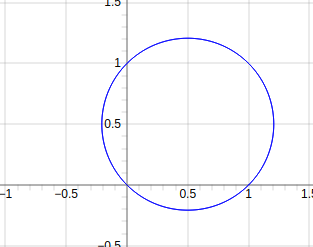
\includegraphics[width=5cm]{3H-7.8-joe.ayoub.INF.png}
	\end{figure}
\end{itemize}

\begin{thebibliography}{999}
%\bibitem{a} Referentie
\end{thebibliography}
\end{document} 
